% Options for packages loaded elsewhere
\PassOptionsToPackage{unicode}{hyperref}
\PassOptionsToPackage{hyphens}{url}
%
\documentclass[
]{article}
\usepackage{amsmath,amssymb}
\usepackage{iftex}
\ifPDFTeX
  \usepackage[T1]{fontenc}
  \usepackage[utf8]{inputenc}
  \usepackage{textcomp} % provide euro and other symbols
\else % if luatex or xetex
  \usepackage{unicode-math} % this also loads fontspec
  \defaultfontfeatures{Scale=MatchLowercase}
  \defaultfontfeatures[\rmfamily]{Ligatures=TeX,Scale=1}
\fi
\usepackage{lmodern}
\ifPDFTeX\else
  % xetex/luatex font selection
\fi
% Use upquote if available, for straight quotes in verbatim environments
\IfFileExists{upquote.sty}{\usepackage{upquote}}{}
\IfFileExists{microtype.sty}{% use microtype if available
  \usepackage[]{microtype}
  \UseMicrotypeSet[protrusion]{basicmath} % disable protrusion for tt fonts
}{}
\makeatletter
\@ifundefined{KOMAClassName}{% if non-KOMA class
  \IfFileExists{parskip.sty}{%
    \usepackage{parskip}
  }{% else
    \setlength{\parindent}{0pt}
    \setlength{\parskip}{6pt plus 2pt minus 1pt}}
}{% if KOMA class
  \KOMAoptions{parskip=half}}
\makeatother
\usepackage{xcolor}
\usepackage[margin=1in]{geometry}
\usepackage{graphicx}
\makeatletter
\def\maxwidth{\ifdim\Gin@nat@width>\linewidth\linewidth\else\Gin@nat@width\fi}
\def\maxheight{\ifdim\Gin@nat@height>\textheight\textheight\else\Gin@nat@height\fi}
\makeatother
% Scale images if necessary, so that they will not overflow the page
% margins by default, and it is still possible to overwrite the defaults
% using explicit options in \includegraphics[width, height, ...]{}
\setkeys{Gin}{width=\maxwidth,height=\maxheight,keepaspectratio}
% Set default figure placement to htbp
\makeatletter
\def\fps@figure{htbp}
\makeatother
\setlength{\emergencystretch}{3em} % prevent overfull lines
\providecommand{\tightlist}{%
  \setlength{\itemsep}{0pt}\setlength{\parskip}{0pt}}
\setcounter{secnumdepth}{-\maxdimen} % remove section numbering
\ifLuaTeX
  \usepackage{selnolig}  % disable illegal ligatures
\fi
\IfFileExists{bookmark.sty}{\usepackage{bookmark}}{\usepackage{hyperref}}
\IfFileExists{xurl.sty}{\usepackage{xurl}}{} % add URL line breaks if available
\urlstyle{same}
\hypersetup{
  pdftitle={CS 532 EC 0.2 - ODU CS Linux},
  pdfauthor={Kimberley Cossey},
  hidelinks,
  pdfcreator={LaTeX via pandoc}}

\title{CS 532 EC 0.2 - ODU CS Linux}
\author{Kimberley Cossey}
\date{2024-01-15}

\begin{document}
\maketitle

\hypertarget{part-1---setting-up-directory-file-and-permissions}{%
\subsection{\texorpdfstring{\textbf{Part \#1 - Setting up directory,
file, and
permissions}}{Part \#1 - Setting up directory, file, and permissions}}\label{part-1---setting-up-directory-file-and-permissions}}

\hypertarget{creating-a-course-directory-text-file}{%
\subsubsection{Creating a course directory \& text
file}\label{creating-a-course-directory-text-file}}

I named my class directory \texttt{websci\_202401} to match the names I
use on my regular computer. I forgot to include the course number in the
title like you suggested, so I will need to go back and edit the
directory name when I figure out how to do that.

Using the \texttt{nano} command took me to a new screen to make the
\texttt{test.txt} file. I made a mistake when I created the file - I hit
``enter'' after typing the last class. I didn't know how to fix the file
after I had saved it, so my line counts and some of my sorting commands
had an extra blank line.

\begin{figure}
\centering
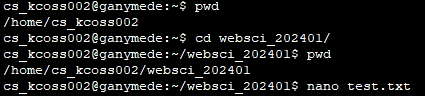
\includegraphics{linux_cmd_mkdir.png}
\caption{\texttt{mkdir} \& \texttt{nano} commands}
\end{figure}

\hypertarget{permissions}{%
\subsubsection{Permissions}\label{permissions}}

I forgot to do this when I created the file. I was able to fix it later
in the process.

\begin{figure}
\centering
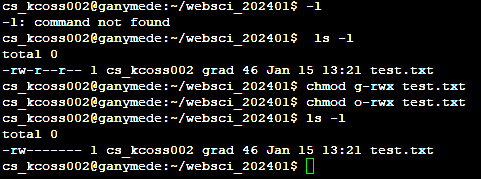
\includegraphics{linux_cmd_permissions.png}
\caption{\texttt{chmod} view and edit}
\end{figure}

\hypertarget{part-2---command-descriptions}{%
\subsection{\texorpdfstring{\textbf{Part \#2 - Command
Descriptions}}{Part \#2 - Command Descriptions}}\label{part-2---command-descriptions}}

\hypertarget{question-1}{%
\subsubsection{Question \#1}\label{question-1}}

\begin{figure}
\centering
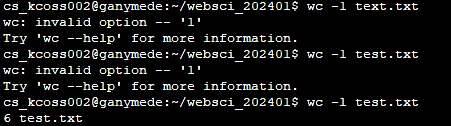
\includegraphics{linux_cmd_1_wcb.png}
\caption{\texttt{wc\ -l}}
\end{figure}

This command printed the number of lines that were in the test file. It
took a couple of tries because I have trouble telling the difference
between 1 and the letter ``l'' when I have to use that font. In my case
I had 6 lines since it counted the blank line.

\hypertarget{question-2}{%
\subsubsection{Question \#2}\label{question-2}}

\begin{figure}
\centering
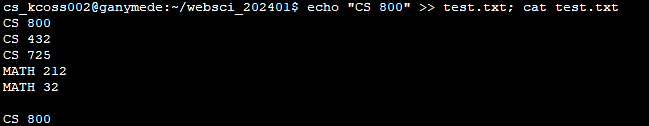
\includegraphics{linux_cmd_2_echo.png}
\caption{\texttt{echo\ "CS\ 800"\ \textgreater{}\textgreater{}\ test.txt;\ cat\ test.txt}}
\end{figure}

This command added ``CS 800'' to a new line at the end of the test file,
so now the test file has 7 lines.

\hypertarget{question-3}{%
\subsubsection{Question \#3}\label{question-3}}

\begin{figure}
\centering
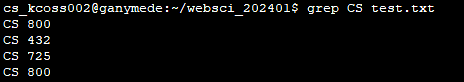
\includegraphics{linux_cmd_3_grepCS.png}
\caption{\texttt{grep\ CS\ test.txt}}
\end{figure}

\texttt{grep} printed the full text of all the lines in the test file
that included the string ``CS''.

\hypertarget{question-4}{%
\subsubsection{Question \#4}\label{question-4}}

\begin{figure}
\centering
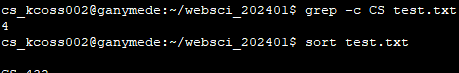
\includegraphics[width=4.92708in,height=0.80208in]{linux_cmd_4_grepc.png}
\caption{\texttt{grep\ -c\ CS\ test.txt}}
\end{figure}

This command printed the number of lines in the test file that included
the string ``CS''.

\hypertarget{question-5}{%
\subsubsection{Question \#5}\label{question-5}}

\begin{figure}
\centering
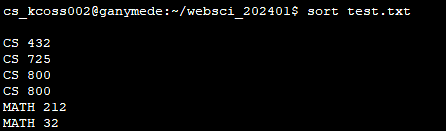
\includegraphics{linux_cmd_5_sort.png}
\caption{\texttt{sort\ test.txt}}
\end{figure}

The basic sort command sorted the lines in the text file by alphabetical
order of the first letter, then by ascending order of the first digit of
the class number, and finally then showed the full text of the file. It
looks like the blank line was sorted to the top.

\hypertarget{question-6}{%
\subsubsection{Question \#6}\label{question-6}}

\begin{figure}
\centering
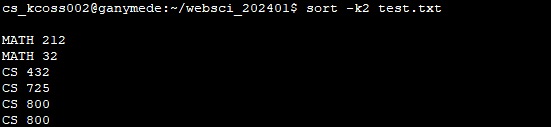
\includegraphics{linux_cmd_6_sortk2.png}
\caption{\texttt{sort\ -k2\ test.txt}}
\end{figure}

Adding the \texttt{-k2} sorted the lines in the file by reverse
alphabetical order, but still sorted the first digit of the class number
as ascending (as in, it didn't reverse sort the first digit from 9 to
1). The blank line is still sorted to the top.

\hypertarget{question-7}{%
\subsubsection{Question \#7}\label{question-7}}

\begin{figure}
\centering
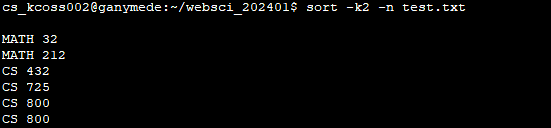
\includegraphics{linux_cmd_7_sortk2n.png}
\caption{\texttt{sort\ -k2\ -n\ test.txt}}
\end{figure}

Adding the \texttt{-n} sorted the lines in the file by reverse
alphabetical order, then sorted the class numbers ascending by their
full numeric value (it finally recognized that 32 was less than 212).

\hypertarget{question-8}{%
\subsubsection{Question \#8}\label{question-8}}

\begin{figure}
\centering
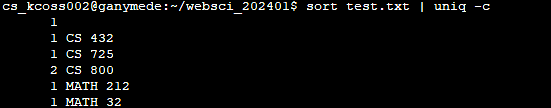
\includegraphics{linux_cmd_8_sortuniq.png}
\caption{\texttt{sort\ test.txt\ \textbar{}\ uniq\ -c}}
\end{figure}

Adding the \texttt{uniq\ -c} command sorted the lines in alphabetical
order, then by full numerical value of the classes. It also returned the
number of lines that contained (or maybe exactly matched) each string.
It shows that there are 2 lines that have the string CS 800, so this
would be a good way to check for duplicates in longer files.

\hypertarget{references}{%
\subsection{\texorpdfstring{\textbf{References}}{References}}\label{references}}

\hypertarget{basic-linux-commands}{%
\subsubsection{Basic Linux commands}\label{basic-linux-commands}}

\begin{itemize}
\tightlist
\item
  \url{https://www.digitalocean.com/community/tutorials/linux-commands}
\end{itemize}

\hypertarget{creating-directories-files}{%
\subsubsection{Creating directories \&
files}\label{creating-directories-files}}

\begin{itemize}
\item
  \url{https://www.redhat.com/sysadmin/create-delete-files-directories-linux}
\item
  \url{https://www.freecodecamp.org/news/how-to-save-and-exit-nano-in-terminal-nano-quit-command/}
\end{itemize}

\hypertarget{how-to-do-permissions}{%
\subsubsection{How to do permissions}\label{how-to-do-permissions}}

\begin{itemize}
\tightlist
\item
  \url{https://www.cs.odu.edu/~zeil/cs252/latest/Public/protection/index.html}
\end{itemize}

\end{document}
